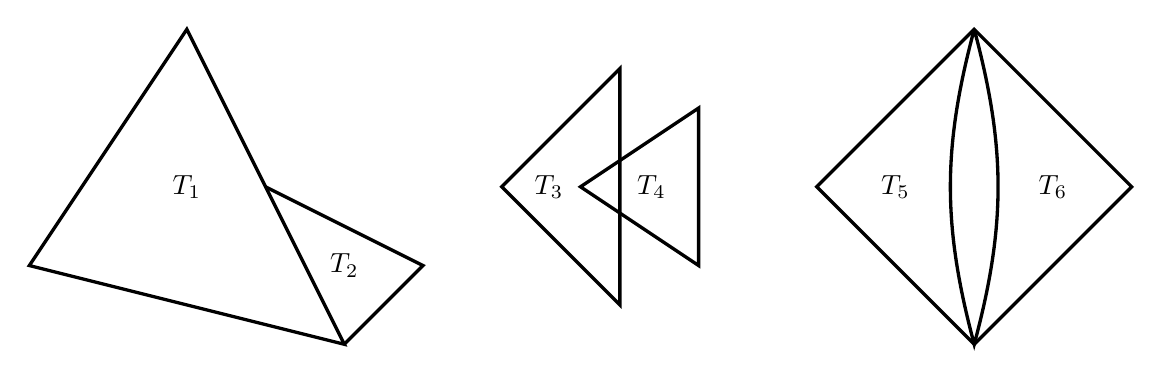
\begin{tikzpicture}
	\def \angle{15}
	\draw[very thick] (0, 0) -- (2, 3) -- (4, -1) -- cycle;
	\draw[very thick] (4, -1) -- (5, 0) -- (3, 1);
	%\\
	\draw[very thick] (6, 0+1) -- (7.5, 1.5+1) -- (7.5, -1.5+1) -- cycle;
	\draw[very thick] (7, 0+1) -- (8.5, 1+1) -- (8.5, -1+1) -- cycle;
	%
	\draw[very thick] (10, 1) -- (12, 3) -- (14, 1) -- (12, -1) -- cycle;
	\draw[very thick] (12, 3) to [out=270+\angle,in=90-\angle] (12, -1) to [out=90+\angle,in=270-\angle] (12, 3);
	\node[] at (2, 1)   (a) {$T_1$};
	\node[] at (4, 0)   (b) {$T_2$};
	\node[] at (6.6, 1)   (c) {$T_3$};
	\node[] at (7.9, 1)   (d) {$T_4$};
	\node[] at (11, 1)   (a) {$T_5$};
	\node[] at (13, 1)   (a) {$T_6$};
\end{tikzpicture}